\subsection{Call Signs}
\label{subsec:call-signs}

In the world of amateur radio, call signs are like your personal identifier—your radio name, if you will. They are unique to each operator and are used to identify who is transmitting. Let’s dive into the rules and formats for these call signs, and maybe have a little fun along the way.

\subsubsection*{Vanity Call Sign Rules}
Ever wanted to pick your own call sign? Well, under the vanity call sign rules, you can! Any licensed amateur, regardless of their license class, can select a desired call sign. That’s right, whether you’re a Technician, General, or Extra class operator, you can choose a call sign that resonates with you. This is a great way to personalize your presence on the airwaves. Just remember, the call sign you choose must still follow the FCC’s format rules.

\subsubsection*{Call Sign Formats}
Now, let's talk about the structure of these call signs. In the United States, amateur radio call signs follow specific format rules based on the license class and region. Here's how they break down:

\begin{itemize}
    \item \textbf{Prefix}: 1 or 2 letters, starting with K, N, or W (and some special cases with AA-AL, KA-KZ, NA-NZ, WA-WZ)
    \item \textbf{Region Number}: A single digit (0-9) indicating the geographic region\footnote{https://www.radioqth.net/vanity/SeqCallSystem}
    \item \textbf{Suffix}: 1 to 3 letters
\end{itemize}

For Technician class operators, the call sign typically follows formats like:
\begin{itemize}
    \item 2x3 format: Two-letter prefix, one number, three-letter suffix (e.g., \texttt{KF1XXX})
    \item 1x3 format: One-letter prefix, one number, three-letter suffix (e.g., \texttt{K1XXX})
\end{itemize}

The length of the suffix can indicate license class:
\begin{itemize}
    \item 2-letter suffix (1x2): Usually reserved for Extra class
    \item 3-letter suffix (1x3 or 2x3): Common for Technician and General class
\end{itemize}

\begin{figure}[h]
    \centering
    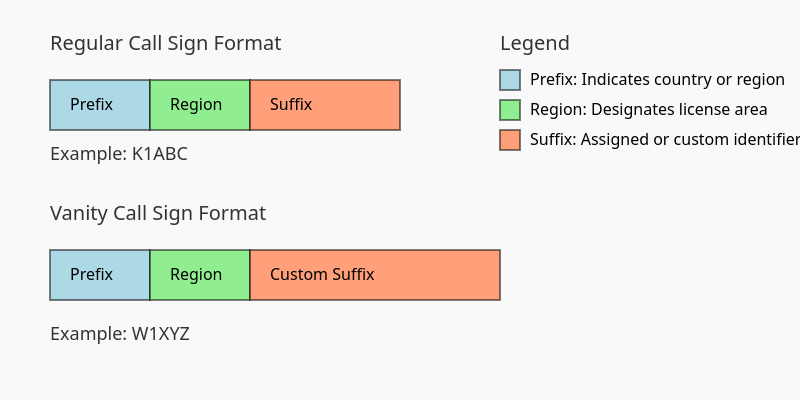
\includegraphics[width=0.8\textwidth]{tech/images/call-sign-structure.png}
    \caption{Structure of an Amateur Radio Call Sign}
    \label{fig:call-sign-structure}
    % Diagram showing the structure of a typical amateur radio call sign.
\end{figure}

\begin{table}[h]
    \centering
    \begin{tabular}{|l|l|l|}
        \hline
        \textbf{Format} & \textbf{Example} & \textbf{Typical Class} \\
        \hline
        1x2 & W1XX & Extra \\
        1x3 & K1XXX & General/Tech \\
        2x3 & KF1XXX & Tech/General \\
        \hline
    \end{tabular}
    \caption{Common Call Sign Formats}
    \label{tab:call-sign-formats}
\end{table}

\subsubsection*{Questions}

\begin{tcolorbox}[colback=gray!10!white,colframe=black!75!black,title={T1C02}]
    Who may select a desired call sign under the vanity call sign rules?
    \begin{enumerate}[label=\Alph*),noitemsep]
        \item Only a licensed amateur with a General or Amateur Extra Class license
        \item Only a licensed amateur with an Amateur Extra Class license
        \item Only a licensed amateur who has been licensed continuously for more than 10 years
        \item \textbf{Any licensed amateur}
    \end{enumerate}
\end{tcolorbox}

Under the vanity call sign rules, any licensed amateur, regardless of their license class, can select a desired call sign. This means even a Technician class operator can choose a call sign that suits them. However, only an Amateur Extra Class operator can select a call sign that is 1x2 or 2x1.

\begin{tcolorbox}[colback=gray!10!white,colframe=black!75!black,title={T1C05}]
    Which of the following is a valid Technician class call sign format?
    \begin{enumerate}[label=\Alph*),noitemsep]
        \item \textbf{KF1XXX}
        \item KA1X
        \item W1XX
        \item All these choices are correct
    \end{enumerate}
\end{tcolorbox}

The correct format for a Technician class call sign is \texttt{KF1XXX}. This format includes a prefix (\texttt{KF}), a number (\texttt{1}), and a suffix (\texttt{XXX}). The other options either do not follow the correct format or are incomplete. Therefore, the correct answer is \textbf{A}.
